
% \chapter{ANN - Artificial Neural Networks}
% \section{Basic Architecture}

\chapter{DNN --- Deep Neural Networks}
\section{ANN --- Artificial Neural Networks}
\section{Basic Architecture}

\section{NN Layers}
\subsection{Linear Layers}
\subsubsection{Linear}
\subsubsection{Bi-Linear}

\subsection{Convolution Layers}
\subsubsection{Convoltion operation}
\begin{equation} \label{eq:conv_operation}
    \text{out}(N_i, C_{\text{out}_j}) = \text{bias}(C_{\text{out}_j}) +
    \sum_{k = 0}^{C_{in} - 1} \text{weight}(C_{\text{out}_j}, k)
    \star \text{input}(N_i, k)
\end{equation}

Both the weights and bias parameters are learnable during the training
process of the network.

\subsubsection{Convolutional Layer Parameters}
\subsection*{Kernel}
A kernel, or a filter, is a set of values that convolves with
the input feature map
as part of the convolutional neural network.
The convolution layer takes the kernel as one operand,
and ``slides'' it over the second operand.
As seen in Equation~\ref{eq:conv_operation},
the convolution operation, sums the dot product of two operands
over the total number of weight values in the kernel.

\begin{figure}[H]
    \centering
    \begin{tikzpicture}[scale=.5,every node/.style={minimum size=1cm}, on grid]
        \draw[fill=base02a,opacity=0.4] (0,0) rectangle (3,3);
        \draw[draw=base03,thick] (0,0) grid (3,3);
        \node (00) at (0.5,2.5) {\tiny 0};
        \node (01) at (1.5,2.5) {\tiny 1};
        \node (02) at (2.5,2.5) {\tiny 2};
        \node (10) at (0.5,1.5) {\tiny 3};
        \node (11) at (1.5,1.5) {\tiny 4};
        \node (12) at (2.5,1.5) {\tiny 5};
        \node (20) at (0.5,0.5) {\tiny 6};
        \node (21) at (1.5,0.5) {\tiny 7};
        \node (22) at (2.5,0.5) {\tiny 8};
    \end{tikzpicture}
\end{figure}

The kernel above, is of size \( \left( \left[ 3, 3 \right] \right) \).
Presenting it as a 4D-Tensor, would give: \( \left( N, C, k_{H}, k_{W} \right)  = \left( \left[ 1, 1, 3, 3 \right] \right)  \)

\subsection*{Stride}
The stride parameter controls the steps in which the kernel
moves across the input feature map.
It takes two values, \( \left( \left[ s_{H}, s_{W} \right] \right) \),
where \( H_{s}, W_{s} \) are the integer step values for the
height and the width movements across the input feature map.

\begin{figure}[H]
    \centering
    \begin{tikzpicture}[scale=.5,every node/.style={minimum size=1cm}, on grid]
        \begin{scope}[xshift=0,yshift=0cm]
            \begin{scope}[xshift=0cm,yshift=0cm]
                \draw[draw=base03,fill=blue,thick] (0,0) grid (5,5) rectangle (0,0);
                \draw[fill=base02a, opacity=0.4] (0,2) rectangle (3,5);
            \end{scope}
            % \begin{scope}[xshift=7cm,yshift=1.5cm]
            %     \draw[draw=base03,fill=cyan,thick] (0,0) grid (2,2) rectangle (0,0);
            % \end{scope}
        \end{scope}
        \draw[draw=base03, ->, thick] (2.6,3.5) to  (4.5,3.5);
        \draw[draw=base03, ->, thick] (1.5,2.4) to (1.5,0.5);
        % \draw[draw=base03, ->, thick] (5.25, 2.5) to (6.75, 2.5);
        % \begin{scope}[xshift=12cm,yshift=0cm]
        %     \begin{scope}[xshift=0cm,yshift=0cm]
        %         \draw[draw=base03,fill=blue,thick] (0,0) grid (5,5) rectangle (0,0);
        %         \draw[fill=base02, opacity=0.4] (0,2) rectangle (3,5);
        %     \end{scope}
        %     \begin{scope}[xshift=7cm,yshift=1cm]
        %         \draw[draw=base03,fill=cyan,thick] (0,0) grid (3,3) rectangle (0,0);
        %         \draw[draw=base03] (1,0) -- (2,1) -- (2,0) -- (1,1);
        %         \draw[draw=base03] (0,1) -- (1,2) -- (1,1) -- (0,2);
        %         \draw[draw=base03] (1,1) -- (2,2) -- (2,1) -- (1,2);
        %         \draw[draw=base03] (2,1) -- (3,2) -- (3,1) -- (2,2);
        %         \draw[draw=base03] (1,2) -- (2,3) -- (2,2) -- (1,3);
        %     \end{scope}
        %     \begin{scope}[xshift=12cm,yshift=1.5cm]
        %         \draw[draw=base03,fill=cyan,thick] (0,0) grid (2,2) rectangle (0,0);
        %     \end{scope}
        % \end{scope}
        % \draw[draw=base03, ->, thick] (14.6,3.5) to  (15.5,3.5);
        % \draw[draw=base03, ->, thick] (15.6,3.5) to  (16.5,3.5);
        % \draw[draw=base03, ->, thick] (13.5,2.4) to (13.5,1.5);
        % \draw[draw=base03, ->, thick] (13.5,1.4) to (13.5,0.5);
        % \draw[draw=base03, ->, thick] (17.25, 2.5) to (18.75, 2.5);
        % \draw[draw=base03, ->, thick] (22.25, 2.5) to (23.75, 2.5);
    \end{tikzpicture}
    \caption{(a) Mel Filter-Bank representation}
\end{figure}

\begin{figure}[H]
    \centering
    \begin{tikzpicture}[scale=.5,every node/.style={minimum size=1cm}, on grid]
        \tikzmath{
            let \strt = 0;
            let \stp = 7;
        }

        \draw[draw=base03,fill=blue,thick] (\strt,\strt) grid (\stp,\stp) rectangle (0,0);
        \draw[fill=base02a, dashed, opacity=0.4] (\strt-1,\strt-1) grid (\stp+1,\stp+1);
        % \draw[fill=base02a, opacity=0.4] (0,2) rectangle (3,5);
        % \draw[draw=base03, ->, thick] (1.5,2.4) to (1.5,0.5);
    \end{tikzpicture}
    \caption{(a) Mel Filter-Bank representation}
\end{figure}


\begin{figure}[H]
    \centering
    \subfloat[\label{mel_fb_ref}]{
        \centering
        \begin{tikzpicture}[scale=.35,every node/.style={minimum size=1cm},
                on grid]
            \draw[fill=blue] (0,0) rectangle (5,5);
            \draw[draw=base03, thick] (0,0) grid (5,5);
            \draw[fill=base02, opacity=0.4] (0,2) rectangle (3,5);
            \draw[step=10mm, base03, thick] (0,2) grid (3,5);
            \draw[draw=base03, ->, thick] (2.6,3.5) to  (3.5,3.5);
            \draw[draw=base03, ->, thick] (3.6,3.5) to  (4.5,3.5);
            \draw[draw=base03, ->, thick] (1.5,2.4) to  (1.5,1.5);
            \draw[draw=base03, ->, thick] (1.5,1.4) to  (1.5,0.5);
        \end{tikzpicture}
    }
    \subfloat[\label{mel_fb_ref}]{
        \centering
        \begin{tikzpicture}[scale=.35,every node/.style={minimum size=1cm},
                on grid]
            \draw[fill=blue] (0,0) rectangle (5,5);
            \draw[draw=base03, thick] (0,0) grid (5,5);
            \draw[fill=base02, opacity=0.4] (0,2) rectangle (3,5);
            \draw[step=10mm, base03, thick] (0,2) grid (3,5);
            \draw[draw=base03, ->, thick] (2.5,3.5) to  (4.5,3.5);
            \draw[draw=base03, ->, thick] (1.5,2.5) to  (1.5,0.5);
        \end{tikzpicture}
    }
    \caption{(a) Mel Filter-Bank representation}
\end{figure}

\subsection*{Padding}
Padding is a method of extending the input feature map with
zero values all around in order to control the size dimensions of the
output feature map. This parameter takes a 2D-Tensor in the form of:
\( \left( \left[ p_{H}, p_{W} \right] \right) \), where \( P_{H}, P_{W} \),
describes the padding depth in the height and width dimensions of the
input feature map.

\begin{figure}[H]
    \centering
    \begin{tikzpicture}[scale=.5,every node/.style={minimum size=1cm}, on grid]
        \draw[draw=base03,fill=blue,thick] (0,0) grid (5,5) rectangle (0,0);
        \draw[fill=base02a, dashed, opacity=0.4] (-1,-1) grid (6,6);
        % \draw[fill=base02a, opacity=0.4] (0,2) rectangle (3,5);
        % \draw[draw=base03, ->, thick] (1.5,2.4) to (1.5,0.5);
    \end{tikzpicture}
    \caption{(a) Mel Filter-Bank representation}
\end{figure}

\subsection*{Dilation}
Dilation represents the integer spaces placed between the kernel elements.
For a given dilation value \(d\),
the elements of the kernel are spaced with \(d - 1\) in between.

This parameter takes a 2D-Tensor in the form of:
\( \left( \left[ d_{H}, d_{W} \right] \right) \),
where \( d_{H}, d_{W} \),
describes the \(d - 1 \) spaces in between kernel elements.

\begin{figure}[H]
    \centering
    \subfloat[\label{conv2d_dil1}]{
        \begin{tikzpicture}[scale=.4,every node/.style={minimum size=1cm}, on grid]

            \draw[draw=base03,fill=blue,thick] (0,0) grid (7,7) rectangle (0,0);
            \draw[fill=base02a, dashed, opacity=0.4] (-1,-1) grid (8,8);

            \foreach \x in {0,1,2} {
                    \foreach \y in {4,5,6} {
                            \draw[fill=base02a, opacity=0.4] (\x,\y) rectangle (\x+1,\y+1);
                            % \node at (\x,\y) [circle,fill=black] {};
                            %this way circle of nodes will not be transformed
                        }
                }
            % \draw[draw=base03, ->, thick] (2.5,2.4) to (2.5,0.5);
            \draw[draw=base03, ->, thick] (1.5,5.5) to  (3.5,5.5);
            \draw[draw=base03, ->, thick] (1.5,5.5) to  (1.5,3.5);
        \end{tikzpicture}
    }
    \subfloat[\label{conv2d_dil2}]{
        \begin{tikzpicture}[scale=.4,every node/.style={minimum size=1cm}, on grid]
            \draw[draw=base03,fill=blue,thick] (0,0) grid (7,7) rectangle (0,0);
            \draw[fill=base02a, dashed, opacity=0.4] (-1,-1) grid (8,8);

            \foreach \x in {0,2,4} {
                    \foreach \y in {2,4,6} {
                            \draw[fill=base02a, opacity=0.4] (\x,\y) rectangle (\x+1,\y+1);
                            % \node at (\x,\y) [circle,fill=black] {};
                            %this way circle of nodes will not be transformed
                        }
                }
            % \draw[draw=base03, ->, thick] (2.5,2.4) to (2.5,0.5);
            \draw[draw=base03, ->, thick] (2.5,4.5) to  (5.5,4.5);
            \draw[draw=base03, ->, thick] (2.5,4.5) to  (2.5,1.5);
        \end{tikzpicture}
    }
    % \subfloat[\label{conv2d_dil3}]{
    %     \begin{tikzpicture}[scale=.4,every node/.style={minimum size=1cm}, on grid]
    %         \draw[draw=base03,fill=blue,thick] (0,0) grid (9,9) rectangle (0,0);
    %         \draw[fill=base02a, dashed, opacity=0.4] (-1,-1) grid (10,10);

    %         \foreach \x in {0,3,6} {
    %             \foreach \y in {2,5,8} {
    %                 \draw[fill=base02a, opacity=0.4] (\x,\y) rectangle (\x+1,\y+1);
    %             }
    %         }
    %         \draw[draw=base03, ->, thick] (3.5,5.5) to  (5.5,5.5);
    %         \draw[draw=base03, ->, thick] (3.5,5.5) to  (3.5,3.5);
    %     \end{tikzpicture}
    % }
    \caption{(a) Mel Filter-Bank representation}
\end{figure}

\subsubsection{Convolutional Layer Output}
A convolutional layer,
after convolving a kernel with an input tensor,
outputs a feature map. The output feature map dimensions
are set by the different parameters of the convolutional layer.

The padding \( p_{H}, p_{W} \) increases the height and width of
the output feature map, while the stride \( s_{H}, s_{W} \)
and dilation \( d_{H}, d_{W} \) shrink it.

\begin{align}
    H_{out} = & \left\lfloor\frac{H_{in}  + 2 \times p_{_{H}} - d_{_{H}}
    \times (k_{_{H}} - 1) - 1}{s_{_{H}}} + 1\right\rfloor                \\
    W_{out} = & \left\lfloor\frac{W_{in}  + 2 \times p_{_{W}} - d_{_{W}}
        \times (k_{_{W}} - 1) - 1}{s_{_{W}}} + 1\right\rfloor
\end{align}

\begin{figure}[H]
    \centering
    \begin{tikzpicture}[scale=.5,every node/.style={minimum size=1cm}, on grid]
        \begin{scope}[xshift=0,yshift=0cm]
            \begin{scope}[xshift=0cm,yshift=0cm]
                \draw[draw=base03,fill=blue,thick] (0,0) grid (5,5) rectangle (0,0);
                \draw[fill=base02, opacity=0.4] (0,2) rectangle (3,5);
            \end{scope}
            \begin{scope}[xshift=7cm,yshift=1.5cm]
                \draw[draw=base03,fill=cyan,thick] (0,0) grid (2,2) rectangle (0,0);
            \end{scope}
        \end{scope}
        \draw[draw=base03, ->, thick] (2.6,3.5) to  (4.5,3.5);
        \draw[draw=base03, ->, thick] (1.5,2.4) to (1.5,0.5);
        \draw[draw=base03, ->, thick] (5.25, 2.5) to (6.75, 2.5);
    \end{tikzpicture}
    \caption{(a) Mel Filter-Bank representation}
\end{figure}



\subsection{Recurrent Layers}
\subsubsection{LSTM}
\subsubsection{BLSTM}
\subsubsection{RNN}

\subsection{Transformer Layers}
\subsubsection{Transformer}
\subsubsection{Transformer-Encoder}
\subsubsection{Transformer-Decoder}


\section{NN Function Layers}
\subsection{Non-linear Activations Functions}
Basic neuron model is not capable of doing much
when it comes to non-linearity decisions.



\subsubsection{ReLU --- Rectified Linear Unit}
This activation function rectifies all the negative
values presented in the output feature map, resulted
from the previous in-line CNN layer.

Applying the ReLU activation function
actually means, in other words, evaluating the following equation: \(ReLU(x) = {\left(x\right)}^{+} = \max(0, x)\)

\begin{figure}[H]
    \centering
    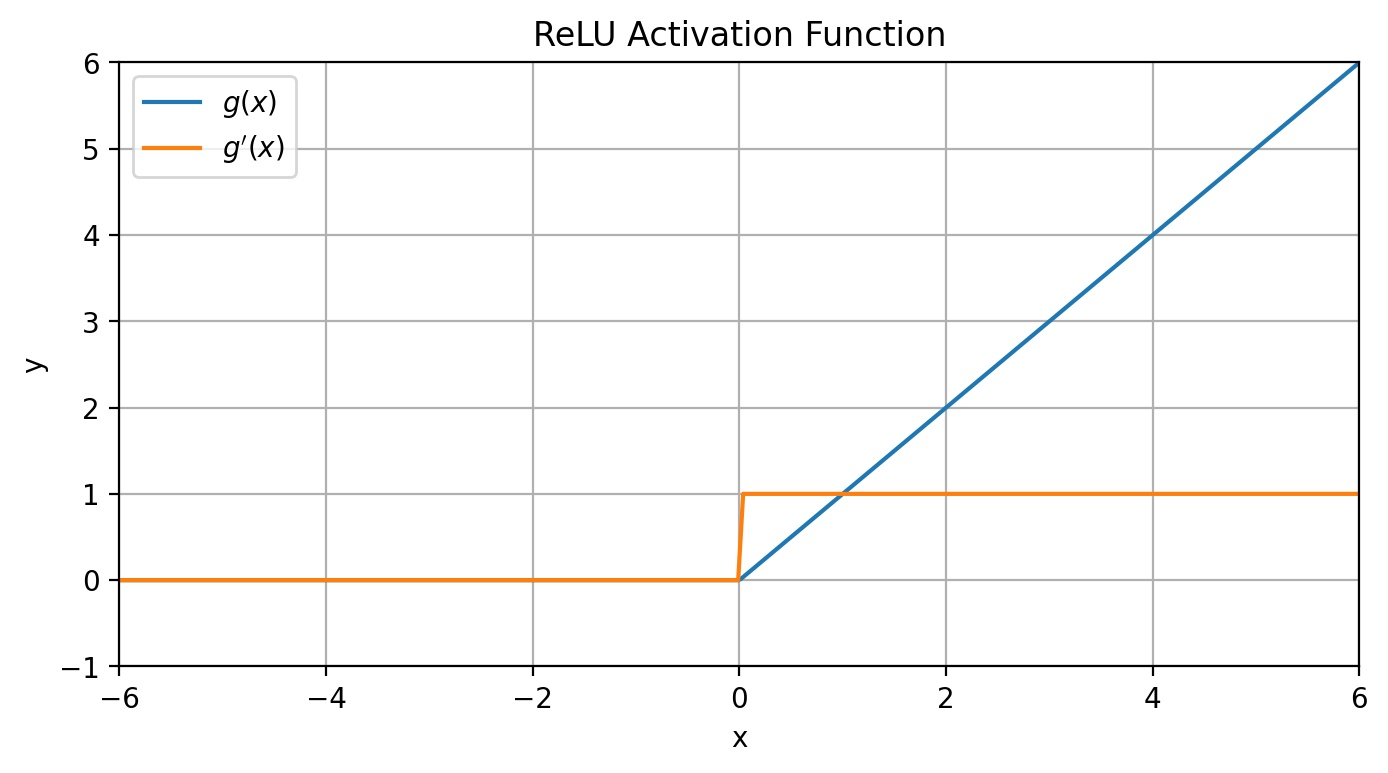
\includegraphics[width=0.75\linewidth]{ANN/images/relu}
    \caption{ReLU activation function and its derivativ}\label{fig:relu_af}
\end{figure}

% \input{images/relu}

\subsubsection{LeakyReLU}
A problem that arises whenever a
ReLU activation function is used within a neural-network
is during the training process.
The back-propagation operation
works on the derivatives of the activation functions.
A ReLU function, clamps all the negative values,
which means, a constant zero value for any input value,
lower than 0. Thus, the derivative of the function
for negative \(x\) values is constant 0 as well.

This kind of behavior, although very simple to implement,
is undesirable and can lead to the nulling of large
sections of the neural network neurons during training.

A small modification to the
ReLU function can help overcome that
problem very easily, while maintaining
the ``same'' characteristics of the
original ReLU function.

By introducing a small negative slope,
the activation function outputs are not pure zeroes.
On top of that, derivatives are also not zero. In that
way, a dying ReLU is prevented.

\begin{figure}[H]
    \centering
    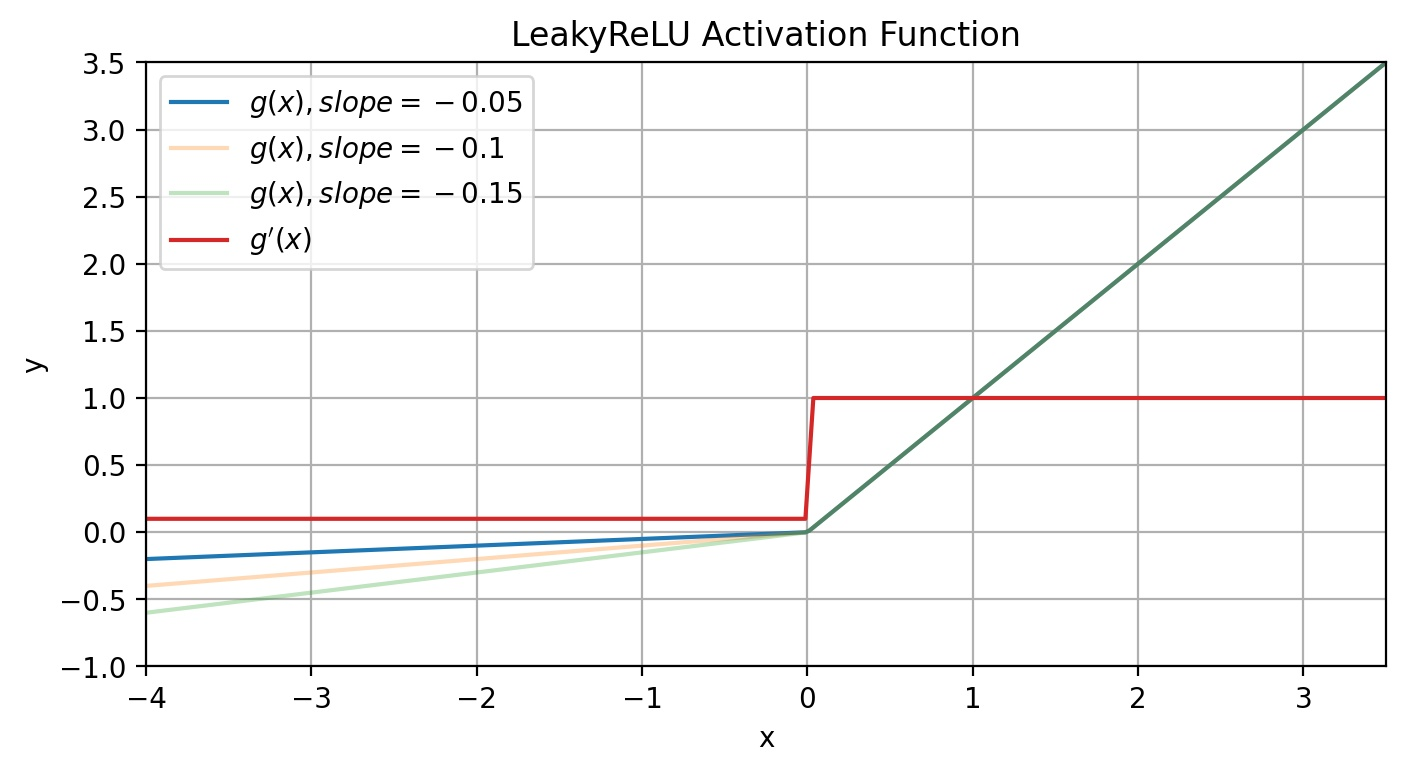
\includegraphics[width=0.75\linewidth]{ANN/images/leakyrelu}
    \caption{Leaky-ReLU activation function and its derivative}\label{fig:leakyrelu_af}
\end{figure}

\subsubsection{Sigmoid}
Another activation function that is commonly used,
is the Sigmoid function. This function is unique
in the matter that it is bounded between \((0, 1)\),
and both the function and its derivate are continuous.

Sigmoid activation functions are usually in use whenever
a network is designed to classify and predict
values between 0 and 1.

An additional advantage of the Sigmoid function is the
fact that its derivative can be
evaluated as \(g(x)(1-g(x))\), which makes it very
efficient in terms of computation efforts, as the result calculated
while forward propagating through the network, is
used in the back-propagation training process.
\begin{figure}[H]
    \centering
    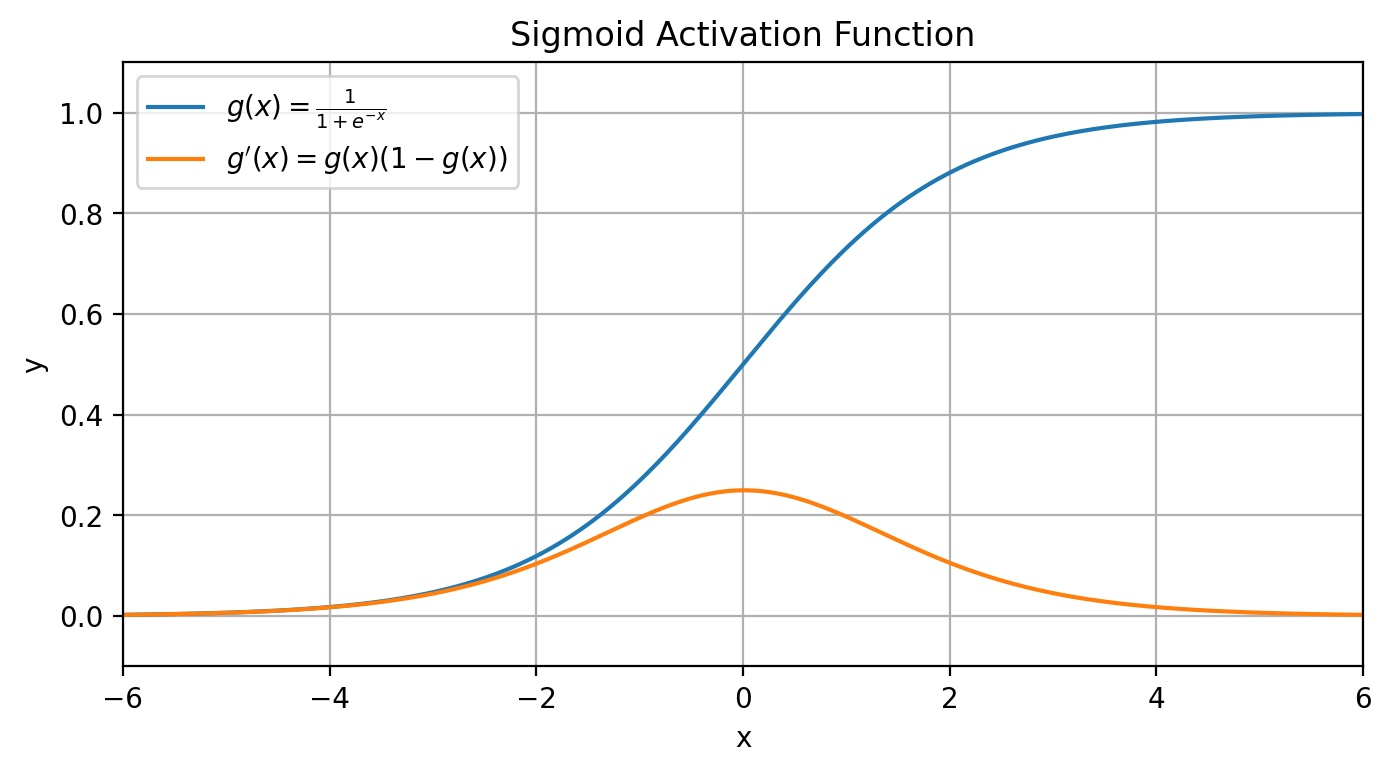
\includegraphics[width=0.75\linewidth]{ANN/images/sigmoid}
    \caption{Sigmoid activation function and its derivative}\label{fig:sigmoid_af}
    % \source{Adapted from \citep{ADI_MIMO}}
\end{figure}

\subsubsection{Tanh}
The benefits of using the Sigmoid activation function
were described above.
However, the Sigmoid function characteristics might not
be enough for applications where the difference
between classes is dichotomy. In such cases,
the contrast between predicted classes should be
strongly emphasized.

The Tanh, hyperbolic tangent, activation function
maintains the continuity characteristics of the
Sigmoid function while extending the range limit to
\((-1, 1)\). That said, the derivative of the Tanh
function is very distinctive in the middle, getting
the value of 1.

\begin{figure}[H]
    \centering
    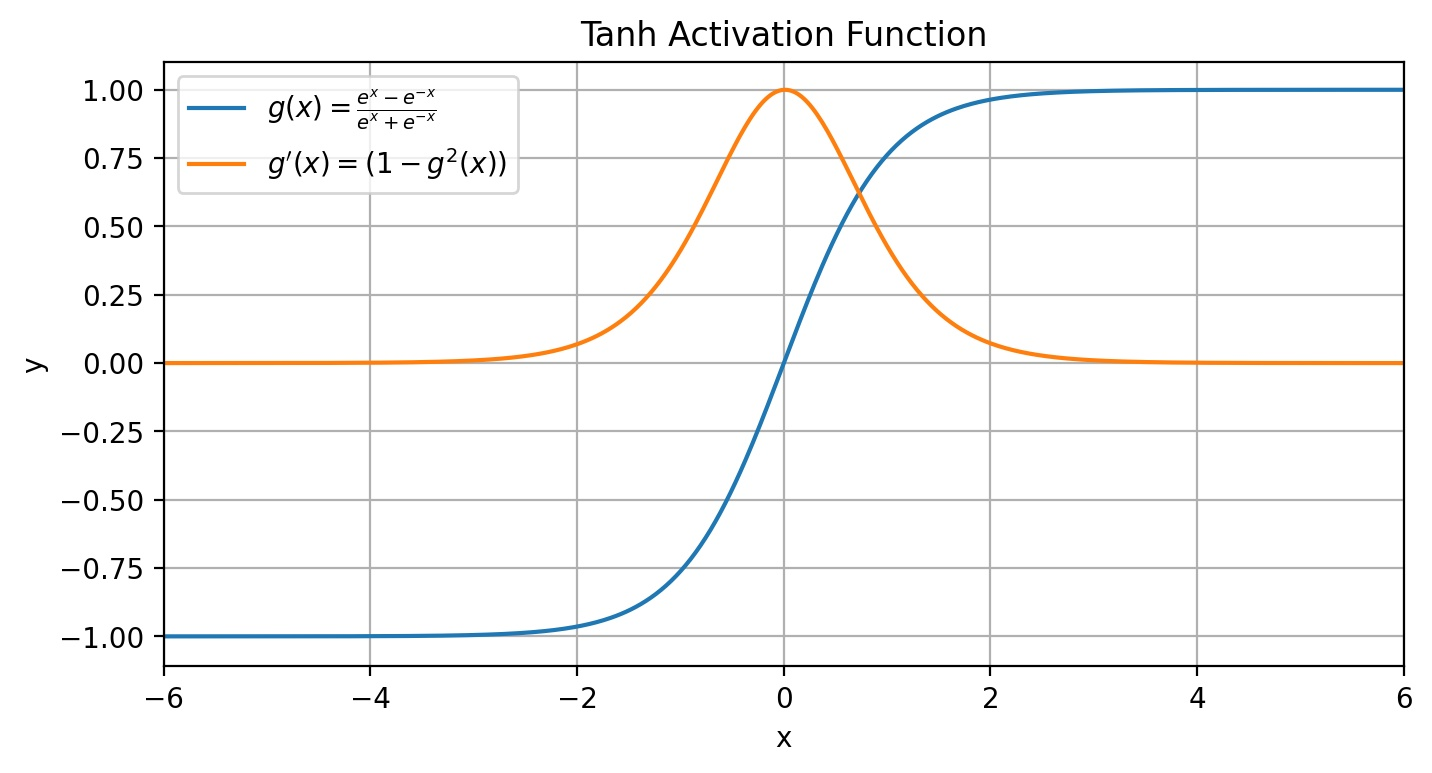
\includegraphics[width=0.75\linewidth]{ANN/images/tanh}
    \caption{Tanh activation function and its derivative}\label{fig:tanh_af}
    % \source{Adapted from \citep{ADI_MIMO}}
\end{figure}

% \subsubsection{Softplus}

\subsection{Normalization Functions}
\subsubsection{Batch-Normalization}

\subsection{Pooling Functions}
\subsubsection{Min-pooling}
\subsubsection{Average-pooling}
\subsubsection{Max-pooling}

\section{Dropout Layers}
\subsubsection{p-Dropout}
To avoid some redundant feature\((s)\) detection by multiple neurons in a network,
a co-adaptation amongst the different neurons in the model should be prevented.
In that way, the NN model is much more effective and uses resources more efficiently.

This holds true especially during training, as described in this paper
\citep{hinton2012improving}.

The idea is to zero-out, arbitrarily, values of
the input feature.
Based on the \emph{Bernoulli distribution}, the probability to zero an element gets the
probability \(p\), while the opposite, non-zeroing probability is set to \(1-p\).

Raising the \(p\) value too high, may lead to an exhaustive training process, thus
a good balance point should be used to overcome the co-adaptation while not missing
useful features. Whenever the training sets are considered large, a small portion
of zeroed elements should be sufficient for satisfactory results.

\subsection{Loss Functions}
\subsubsection{L1 Loss (MAE)}
\subsubsection{L2 Loss (MSE)}
\subsubsection{Cross-Entropy}
\subsubsection{CTC}